\section{Табличные алгоритмы}\label{tabularrlsection}

\subsection{Монте-Карло алгоритм}

Value iteration и Policy iteration имели два ограничения: 1) необходимо уметь хранить табличку размером $| \St |$ в памяти и перебирать все состояния и действия за разумное время 2) должна быть известна динамика среды $p(s' \mid s, a)$. Первое полечим нейронками, а сейчас будем лечить второе: в сложных средах проблема даже не столько в том, чтобы приблизить динамику среды, а в том, что интегралы $\E_{s' \sim p(s' \mid s, a)}$ мы не возьмём в силу огромного числа состояний и сможем только оценивать по Монте-Карло. 
Итак, мы хотим придумать табличный model-free RL-алгоритм: мы можем отправить в среду пособирать траектории какую-то стратегию, и дальше должны проводить итерации алгоритма, используя лишь эти сэмплы траекторий. Иначе говоря, для данного $s$ мы можем выбрать $a$ и получить ровно один сэмпл из очередного $p(s' \mid s, a)$, причём на следующем шаге нам придётся проводить сбор сэмплов именно из $s'$. Как в таких условиях <<решать>> уравнения Беллмана --- неясно.

Рассмотрим самый простой способ превратить Policy Iteration в model-free метод. Давайте очередную стратегию $\pi_k$ отправим в среду, сыграем несколько эпизодов, и будем оценивать $Q^{\pi_k}$ по Монте-Карло:
$$Q^{\pi}(s, a) \approx \frac{1}{N} \sum_{i=0}^N R(\Traj_i), \quad \Traj_i \sim \pi \mid s_0 = s, a_0 = a$$

\needspace{7\baselineskip}
\begin{wrapfigure}{r}{0.35\textwidth}
%\vspace{-0.3cm}
\centering
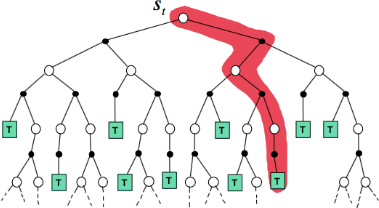
\includegraphics[width=0.3\textwidth]{Images/MC_backup.png}
%\vspace{-0.3cm}
\end{wrapfigure}
Теперь, доиграв эпизод до конца, мы для каждой встретившейся пары $s, a$ в полученной траектории можем посчитать reward-to-go и использовать этот сэмпл для обновления нашей аппроксимации Q-функции --- проведения \emph{Монте-Карло бэкапа} (MC-backup). Такое обновление полностью противоположно по свойствам бэкапу динамического программирования: это <<бэкап ширины один>> бесконечной длины --- мы использовали лишь один сэмпл будущего и при этом заглянули в него на бесконечное число шагов вперёд.

\begin{remark}
Формально, из-за петлей сэмплы являются скоррелированными. Если мы крутимся в петле, а потом в какой-то момент эпизода вышли и получили +1, то сэмплы будут выглядеть примерно так: $\gamma^5, \gamma^4, \gamma^3 \dots$. Причина в том, что мы взяли по несколько сэмплов для одной и той же Монте-Карло оценки (для одной и той же пары $s, a$) из одного и того же эпизода (<<\emph{every-visit}>>); для теоретической корректности следует гарантировать независимость сэмплов, например, взяв из каждого эпизода для каждой пары $s, a$ сэмпл только для первого посещения (<<\emph{first-visit}>>).
\end{remark}

\needspace{7\baselineskip}
\begin{wrapfigure}{l}{0.35\textwidth}
\vspace{-0.3cm}
\centering
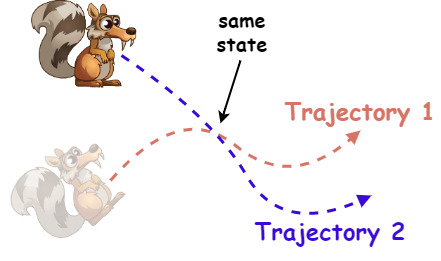
\includegraphics[width=0.3\textwidth]{Images/TrajIntersect.png}
\vspace{-0.3cm}
\end{wrapfigure}

Монте-Карло алгоритм, на первый взгляд, плох примерно всем. Нужно доигрывать игры до конца, то есть алгоритм неприменим в неэпизодичных средах; Монте-Карло оценки также обладают огромной дисперсией, поскольку мы заменили на сэмплы все мат.ожидания, стоящие в мат.ожидании по траекториям; наконец, мы практически перестали использовать структуру задачи. Если мы получили сэмпл +100 в качестве очередного сэмпла для $Q^{\pi}(s, a)$, то мы <<забыли>>, какую часть из этой +100 мы получили сразу же после действия $a$, а какая была получена в далёком будущем --- не использовали разложение награды за эпизод в сумму наград за шаг. Также мы посеяли <<информацию о соединениях состояниях>>: пусть у нас было две траектории (см. рисунок), имевших пересечение в общем состоянии. Тогда для начал этих траекторий мы всё равно считаем, что собрали лишь один сэмпл reward-to-go, хотя в силу марковости у нас есть намного больше информации.

Ещё одна проблема алгоритма: если для некоторых $s, a \colon \pi(a \mid s) \HM= 0$, то мы ничего не узнали об $Q^\pi(s, a)$. А, как было видно в алгоритмах динамического программирования, мы существенно опираемся в том числе и на значения Q-функции для тех действий, которые $\pi$ никогда не выбирает; только за счёт этого мы умеем проводить policy improvement для детерминированных стратегий.

А ещё в таком Монте-Карло алгоритме встаёт вопрос: когда заканчивать оценивание Q-функции и делать шаг Policy Improvement-а? Точное значение $Q^{\pi_k}$ за конечное время мы Монте-Карло оценкой всё равно не получим, и в какой-то момент improvement проводить придётся, с потерей теоретических гарантий. Возникает вопрос: насколько разумно в таких условиях после очередного обновления стратегии начинать расчёт оценочной функции $Q^{\pi_{k+1}}$ <<с нуля>>? Может, имеет смысл проинициализировать как-то приближением $Q^{\pi_k}$, которое хоть и считалось для <<предыдущей>> стратегии и формально содержит сэмплы не из того распределения, но всё-таки их там было аккумулировано много, да и стратегия потенциально поменялась не сильно. Возникает желание усреднять сэмплы с приоритетом более свежих, приходящих из <<правильной>> стратегии; а <<неправильные>> сэмплы, из старой стратегии, всё-таки использовать, но с каким-то маленьким весом. Хочется это как-то делать онлайн, не храня всю историю Монте-Карло оценок.

\subsection{Экспоненциальное сглаживание}

Рассмотрим такую задачу. Нам приходят сэмплы $x_1, x_2 \dots x_n \sim p(x)$. Хотим по ходу получения сэмплов оценивать мат.ожидание случайной величины $x$. Давайте хранить Монте-Карло оценку, усредняя все имеющиеся сэмплы; для этого достаточно пользоваться следующим рекурсивным соотношением:
$$m_{k} \coloneqq \frac{1}{k} \sum_{i=1}^{k} x_i = \frac{k - 1}{k}m_{k-1} + \frac{1}{k}x_{k}$$
Обозначим за $\alpha_k \coloneqq \frac{1}{k}$. Тогда формулу можно переписать так:
$$m_{k} \coloneqq (1 - \alpha_k)m_{k-1} + \alpha_k x_{k}$$

\begin{definition}
\emph{Экспоненциальным сглаживанием} (exponential smoothing) для последовательности $x_1, x_2, x_3 \dots$ будем называть следующую оценку:
$$m_{k} \coloneqq (1 - \alpha_k) m_{k - 1} + \alpha_k x_k,$$
где $m_0$ --- некоторое начальное приближение, последовательность $\alpha_k \in [0, 1]$ --- гиперпараметр. 
\end{definition}

Можно ли оценивать мат.ожидание как-то по-другому? В принципе, любая выпуклая комбинация имеющихся сэмплов будет несмещённой оценкой. В частности, если $\alpha_k > \frac{1}{k}$, то мы <<выдаём>> более свежим сэмплам больший вес. Зададимся таким техническим вопросом: при каких других последовательностях $\alpha_k$ формула позволит оценивать среднее?

\begin{definition}
Будем говорить, что последовательность $\alpha_k \in [0, 1]$ удовлетворяет \emph{условиям Роббинса-Монро} (Robbins-Monro conditions), если:
\begin{equation}\label{RobbinsMonro}
\sum_{k \ge 0} \alpha_k = +\infty, \quad \sum_{k \ge 0} \alpha_k^2 < +\infty.
\end{equation}
\end{definition}

\begin{theoremBox}[label=th:expsmoothingconvergence]{}
Пусть $x_1, x_2 \dots$ --- независимые случайные величины, $\E x_k = m, \mathbb{D} x_k \le C < +\infty$, где $C$ --- некоторая конечная константа. Пусть $m_0$ --- произвольно, а последовательность чисел $\alpha_k \in [0, 1]$ удовлетворяет условиям Роббинса-Монро \eqref{RobbinsMonro}. Тогда экспоненциальное сглаживание 
\begin{equation}\label{expsmoothingtheoremexpr}
m_k \coloneqq (1 - \alpha_k) m_{k-1} + \alpha_k x_k
\end{equation}
сходится к $m$ с вероятностью 1.
\begin{proof}
Без ограничения общности будем доказывать утверждение для $m = 0$, поскольку для сведения к этому случаю достаточно вычесть $m$ из правой и левой части \eqref{expsmoothingtheoremexpr} и перейти к обозначениям $\hat{m_k} \HM\coloneqq m_k - m, \hat{x_k} \HM\coloneqq x_k \HM- m$.

Итак, пусть $\E x_k \HM= 0$. Будем доказывать, что $v_k \HM\coloneqq \E m_k^2 \xrightarrow{k \to \infty} 0$. Для начала возведём обе стороны уравнения \eqref{expsmoothingtheoremexpr} в квадрат:
$$m_{k}^2 = (1 - \alpha_k)^2 m^2_{k-1} + \alpha^2_k x^2_k + 2\alpha_k(1 - \alpha_k)x_km_{k-1}$$
Возьмём справа и слева мат.ожидание:
$$\E m_{k}^2 = (1 - \alpha_k)^2 \E m^2_{k-1} + \alpha^2_k \E x^2_k + 2\alpha_k(1 - \alpha_k)\E (x_k m_{k-1})$$
Последнее слагаемое зануляется, поскольку в силу независимости $\E (x_k m_{k-1}) \HM= \E x_k \E m_{k-1}$, а $\E x_k$ равно нулю по условию. Используя введённое обозначение, получаем такой результат:
\begin{equation}\label{recurrentdispersion}
v_{k} = (1 - \alpha_k)^2 v_{k-1} + \alpha_k^2 \E x_k^2
\end{equation}

Сейчас мы уже можем доказать, что $v_k \HM\le C$. Действительно, сделаем это по индукции. База: $v_0 \HM= 0 \HM\le C$ по определению. Шаг: пусть $v_{k-1} \le C$, тогда
$$v_{k} = (1 - \alpha_k)^2 v_{k-1} + \alpha_k^2 \E x_k^2 \le (1 - \alpha_k)^2 C + \alpha_k^2 C \le C$$
где последнее неравенство верно при любых $\alpha_k \in [0, 1]$.

Особенность дальнейшего доказательства в том, что последовательность $v_k$ вовсе не обязана быть монотонной. Поэтому применим пару фокусов в стиле матана. Сначала раскроем скобки в рекурсивном выражении \eqref{recurrentdispersion}:
$$v_{k} - v_{k-1} = - 2\alpha_k v_{k-1} + \alpha_k^2 (v_{k-1} + \E x_k^2)$$

Мы получили счётное число равенств, проиндексированных $k$. Просуммируем первые $n$ из них:
\begin{equation}\label{expsmoothdisperrec}
v_{n} - v_0 = - 2 \sum_{k = 0}^{n-1} \alpha_k v_k + \sum_{k = 0}^{n-1} \alpha_k^2 (v_k + \E x_k^2)
\end{equation}

Заметим, что $v_0 \HM= 0$, а $v_{n} \HM\ge 0$ по определению как дисперсия. Значит: 
$$2 \sum_{k = 0}^{n-1} \alpha_k v_k \le \sum_{k = 0}^{n-1} \alpha_k^2 (v_k + \E x_k^2)$$
Применяем ограниченность $v_k$ и $\E x_k^2$:
$$2 \sum_{k = 0}^{n-1} \alpha_k v_k \le \sum_{k = 0}^{n-1} \alpha_k^2 (C + C) = 2C \sum_{k = 0}^{n-1} \alpha_k^2$$
Ряд справа сходится при $n \to +\infty$. Значит, сходится и ряд слева. Коли так, имеет предел правая часть \eqref{expsmoothdisperrec}. Значит, имеет предел и левая.

Было доказано, что последовательность $v_k$ имеет предел. Понятно, что он неотрицателен. Допустим, он положителен и отделён от 0, равен некоторому $b \HM> 0$. Возьмём какое-нибудь небольшое $\eps \HM> 0$, так что $b \HM- \eps \HM> 0$. Тогда, начиная с некоторого номера $i$ все элементы последовательности $v_k \HM> b \HM- \eps$ при $k \HM\ge i$. Получим:
$$\sum_{k = 0}^{n-1} \alpha_k v_k \ge \sum_{k = i}^{n-1} \alpha_k v_k \ge (b - \eps) \sum_{k = i}^{n-1} \alpha_k$$
Правая часть неравенства расходится, поскольку мы просили расходимость ряда из $\alpha_k$; но ранее мы доказали сходимость левой части. Значит, предел равен нулю.
\end{proof}
\end{theoremBox}

\subsection{Стохастическая аппроксимация}

Мы научились, можно считать, решать уравнения такого вида:
$$x = \E_{\eps} f(\eps),$$
где справа стоит мат.ожидание по неизвестному распределению $\eps \sim p(\eps)$ от какой-то функции $f$, которую для данного значения сэмпла $\eps$ мы умеем считать. Это просто стандартная задача оценки среднего, для которой мы даже доказали теоретические гарантии сходимости следующего итеративного алгоритма:
$$x_k = (1 - \alpha_k)x_{k-1} + \alpha_k f(\eps), \quad \eps \sim p(\eps)$$

Аналогично у нас есть итеративный алгоритм для решения систем нелинейных уравнений
$$x = f(x),$$
где справа стоит, если угодно, <<хорошая>> функция --- сжатие. Формула обновления в методе простой итерации выглядела вот так:
$$x_k = f(x_{k-1})$$

\begin{definition}
\emph{Стохастическая аппроксимация} (Stochastic approximation) --- задача решения уравнения вида
\begin{equation}\label{stochapproxeq}
x = \E_{\eps} f(x, \eps),
\end{equation}
где справа стоит мат.ожидание по неизвестному распределению от функции, которую при данном сэмпле $\eps$ и некотором значении неизвестной переменной $x$ мы умеем считать. 
\end{definition}

Можно ли объединить идеи метода простой итерации и экспоненциального сглаживания (<<перевзвешанной>> Монте-Карло оценки)? Давайте запустим аналогичный итеративный алгоритм: на $k$-ой итерации подставим текущее приближение неизвестной переменной $x_k$ в правую часть $f(x_k, \eps)$ для $\eps \sim p(\eps)$, но не будем <<жёстко>> заменять $x_{k+1}$ на полученное значение, так как оно является лишь несмещённой оценкой правой части; вместо этого сгладим старое значение $x_k$ и полученный новый <<сэмпл>>:
\begin{equation}\label{stochapprox}
x_k = (1 - \alpha_k)x_{k-1} + \alpha_k f(x_{k-1}, \eps), \quad \eps \sim p(\eps)
\end{equation}

Есть хорошая надежда, что, если функция $f$ <<хорошая>>, распределение $p(\eps)$ не сильно страшное (например, имеет конечную дисперсию, как в теореме о сходимости экспоненциального сглаживания), а $\alpha_k$ удовлетворяют условиям \eqref{RobbinsMonro}, то такая процедура будет в пределе сходиться.

Поймём, почему задача стохастической аппроксимации тесно связана со стохастической оптимизацией. Для этого перепишем формулу \eqref{stochapprox} в альтернативной очень интересной форме:
\begin{equation}\label{stochapproxgrad}
x_k = x_{k-1} + \alpha_k \left( f(x_{k-1}, \eps) - x_{k-1} \right), \quad \eps \sim p(\eps)
\end{equation}
Да это же формула стохастического градиентного спуска! И, видимо, выражение $f(x_{k-1}, \eps) \HM- x_{k-1}$ есть какой-то <<стохастический градиент>>. Стохастический он потому, что это выражение случайно: мы сэмплируем $\eps \sim p(\eps)$; а градиент поскольку он обладает следующим свойством: в точке решения, то есть в точке $x^*$, являющейся решением уравнения \eqref{stochapproxeq}, в среднем его значение равно нулю: 
$$\E_{\eps} \left( f(x^*, \eps) - x^* \right) = 0$$

Это наблюдение будет иметь для нас ключевое значение. В model-free режиме как при оценивании стратегии, когда мы решаем уравнение Беллмана
$$Q^{\pi}(s, a) = \E_{s'} \left[ r(s, a) + \gamma \E_{a'} Q^{\pi}(s', a') \right],$$
так и когда мы пытаемся реализовать Value Iteration и напрямую решать уравнения оптимальности Беллмана
$$Q^*(s, a) = \E_{s'} \left[ r(s, a) + \gamma \max_{a'} Q^*(s', a') \right],$$
мы сталкиваемся в точности с задачей стохастической аппроксимации \eqref{stochapproxeq}! Справа стоит мат.ожидание по недоступному нам распределению, содержимое которого мы, тем не менее, при данном сэмпле $s' \HM\sim p(s' \mid s, a)$ и текущем приближении Q-функции, умеем считать. Возникает идея проводить стохастическую аппроксимацию: заменять правые части решаемых уравнений на несмещённые оценки и сглаживать текущее приближение с получаемыми сэмплами.

Отметим интересный факт: уравнение V*V* \eqref{V*V*}, имеющее вид <<максимум от неизвестного распределения>>
$$V^*(s) = \max_{a} \left[ r(s, a) + \gamma \E_{s'}V^*(s') \right],$$
под данную форму не попадает. И с такими уравнениями мы ничего сделать не сможем. К счастью, нам и не понадобится.

\subsection{Temporal Difference}

% TODO: взгляд через бутстрап

Итак, попробуем применить идею стохастической аппроксимации для решения уравнений Беллмана. На очередном шаге после совершения действия $a$ из состояния $s$ мы получаем значение награды $r \HM\coloneqq r(s, a)$, сэмпл следующего состояния $s'$ и генерируем $a' \HM\sim \pi$, после чего сдвигаем наше текущее приближение $Q^\pi(s, a)$ в сторону сэмпла
$$y \coloneqq r + \gamma Q^\pi(s', a'),$$
который также будем называть \emph{таргетом}\footnote{в англоязычной литературе встречается слово guess --- <<догадка>>; этот таргет имеет смысл наших собственных предположений о том, какое будущее нас ждёт.} (Bellman target). Получаем следующую формулу обновления:

\begin{equation}\label{TDupdate}
Q^\pi_{k+1}(s, a) \leftarrow Q^{\pi}_k(s, a) + \alpha_k \underbrace{\left( \overbrace{r + \gamma Q^{\pi}_k(s', a')}^{\text{\emph{таргет}}} - 
Q^{\pi}_k(s, a) \right)}_\text{\emph{временная разность}} 
\end{equation}

Выражение $r(s, a) + \gamma Q^\pi_k(s', a') - Q^\pi_k(s, a)$ называется \emph{временной разностью} (temporal difference): это отличие сэмпла, который нам пришёл, от текущей оценки среднего.

\needspace{7\baselineskip}
\begin{wrapfigure}{r}{0.35\textwidth}
%\vspace{-0.3cm}
\centering
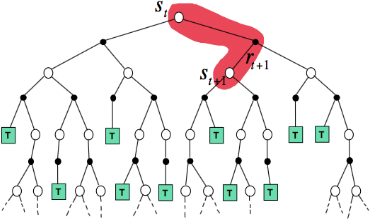
\includegraphics[width=0.3\textwidth]{Images/TD_backup.png}
%\vspace{-0.3cm}
\end{wrapfigure}

Мы таким образом придумали \emph{TD-backup}: обновление, имеющее как ширину, так и длину один. Мы рассматриваем лишь одну версию будущего (один сэмпл) и заглядываем на один шаг вперёд, приближая всё дальнейшее будущее своей собственной текущей аппроксимацией. Этот ход позволяет нам учиться, не доигрывая эпизоды до конца: мы можем обновить одну ячейку нашей Q-функции сразу же после одного шага в среде, после сбора одного перехода $(s, a, r, s', a')$.

Формула \eqref{TDupdate} отличается от Монте-Карло обновлений Q-функции лишь способом построения таргета: в Монте-Карло мы бы взяли в качестве $y$ reward-to-go, когда здесь же используем одношаговое приближение. Поэтому смотреть на эту формулу также можно через интуицию \emph{бутстрапирования} (bootstrapping)\footnote{бутстрэп --- <<ремешки на ботинках>>, происходит от выражения <<потянуть самого себя за ремешки на ботинках и так перелезть через ограду>>. Русскоязычный аналог --- <<тащить самого себя за волосы из болота>>. Наши таргеты построены на принципе такого бутстрапирования, поскольку мы начинаем <<из воздуха>> делать себе сэмплы из уже имеющихся сэмплов.}. Мы хотим получить сэмплы для оценки нашей текущей стратегии $\pi$, поэтому делаем один шаг в среде и приближаем всю оставшуюся награду нашей текущей аппроксимацией среднего. Такой <<псевдосэмпл>> уже не будет являться корректным сэмплом для $Q^{\pi}(s, a)$, но в некотором смысле является <<более хорошим>>, чем то, что у нас есть сейчас, за счёт раскрытия дерева на один шаг и получения информации об $r, s'$. Такое движение нашей аппроксимации в сторону чего-то хоть чуть-чуть более хорошего и позволяет нам чему-то учиться.

\begin{example}
Вы сидите в кафе ($s$) и хотите вернуться домой. Вы прикидываете, что в среднем этой займёт $-Q^\pi(s, a) = 30$ минут. Вы тратите одну минуту ($-r$) на выход из кафе и обнаруживаете пробку ($s'$). За счёт этой новой информации вы можете дать более точную оценку времени до возвращения до дома: $-Q^\pi(s', a') = 40$ минут. Как можно в будущем откорректировать наши прогнозы? Можно засечь время, сколько в итоге заняла поездка --- доиграть эпизод до конца и посчитать Монте-Карло оценку --- а можно уже сделать вывод о том, что случилась некоторая <<временная разность>>, ошибка за один шаг, равная $41 - 30 \HM= 11$ минут. Заменять исходное приближение расстояния от кафе до дома $-Q^\pi(s, a)$ на 41 минуту, конечно же, слишком грубо: но временная разность говорит, что 30 минут было заниженной оценкой и её надо чуть-чуть увеличить.
\end{example}

Обсудим следующий важный технический момент. Какие есть ограничения на переходы $(s, a, r, s', a')$, которые мы можем использовать для обновлений по формуле \eqref{TDupdate}? Пока мы говорили, что мы хотим заниматься оцениванием стратегии $\pi$, и поэтому предлагается, видимо, ею и взаимодействовать со средой, собирая переходы. С точки же зрения стохастической аппроксимации, для корректности обновлений достаточно выполнения всего лишь двух требований:
\begin{itemize}
    \item $s' \sim p(s' \mid s, a)$; если $s'$ приходит из какой-то другой функции переходов, то мы учим Q-функцию для какого-то другого MDP.
    \item $a' \sim \pi(a' \mid s')$; если $a'$ приходит из какой-то другой стратегии, то мы учим Q-функцию для вот этой другой стратегии.
\end{itemize}
Оба этих утверждения вытекают из того, что обновление \eqref{TDupdate} неявно ищет решение уравнения
$$Q(s, a) = \E_{s'} \E_{a'} y$$
как схема стохастической аппроксимации. Поэтому мы будем уделять много внимания тому, из правильных ли распределений приходят данные, которые мы <<скармливаем>> этой формуле обновления. Но и с другой стороны: схема не требует, например, чтобы после $Q^{\pi}(s, a)$ мы обязательно на следующем шаге обновили $Q^{\pi}(s', a')$, ровно как и не говорит ничего о требованиях на распределение, из которого приходят пары $s, a$. Как мы увидим позже, это наблюдение означает, что нам вовсе не обязательно обучаться с онлайн-опыта.

Поскольку довести $Q^{\pi}$ до точного значения с гарантиями мы всё равно не сможем, однажды в алгоритме нам всё равно придётся сделать policy improvement. Что, если мы будем обновлять нашу стратегию $\pi_k(s) \coloneqq \argmax\limits_a Q^{\pi}_k(s, a)$ после каждого шага в среде и каждого обновления Q-функции? Наше приближение Policy Iteration схемы, аналогично ситуации в динамическом программировании, превратится в приближение Value Iteration схемы:
\begin{align*}
y &= r + \gamma Q^{\pi}_k(s', a') = \\
&= r + \gamma Q^{\pi}_k(s', \pi_k(s')) = \\
&= r + \gamma Q^{\pi}_k(s', \argmax_{a'} Q^{\pi}_k(s', a')) = \\
&= r + \gamma \max_{a'} Q^{\pi}_k(s', a')
\end{align*}

Мы получили в точности таргет для решения методом стохастической аппроксимации уравнения оптимальности Беллмана; поэтому для такого случая будем обозначать нашу Q-функцию как аппроксимацию $Q^*$, и тогда наше обновление принимает следующий вид:
\begin{equation}\label{Qlearningupdate}
Q^*_{k+1}(s, a) \leftarrow Q^{*}_k(s, a) + \alpha_k \left( r + \gamma \max_{a'} Q^{*}_k(s', a') - 
Q^{\pi}_k(s, a) \right) 
\end{equation}

\begin{theoremBox}[label=th:TDconvergencetheorem]{Сходимость Q-learning}
Пусть пространства состояний и действий конечны, $Q^*_0(s, a)$ --- начальное приближение, на $k$-ой итерации $Q^*_k(s, a)$ для всех пар $s, a$ строится по правилу
$$Q^*_{k+1}(s, a) \coloneqq Q^*_k(s, a) + \alpha_k(s, a) \left( r(s, a) + \gamma \max_{a'} Q^*_k(s'_k(s, a), a') - Q^*_k(s, a)\right)$$
где $s'_k(s, a) \sim p(s' \mid s, a)$, а $\alpha_k(s, a) \in [0, 1]$ --- случайные величины, с вероятностью один удовлетворяющие для каждой пары $s, a$ условиям Роббинса-Монро:
\begin{equation}\label{TDconvergence}
\sum_{k \ge 1} \alpha_k(s, a) = +\infty \qquad \sum_{k \ge 1} \alpha_k(s, a)^2 < +\infty
\end{equation}
Тогда $Q^*_k$ сходится к $Q^*$ с вероятностью один.
\begin{proof}[Доказательство вынесено в приложение \ref{appendix:qlearning}]
\end{proof}
\end{theoremBox}

В частности, если агент некоторым образом взаимодействует со средой и на $k$-ом шаге обновляет своё текущее приближение $Q^*$ только для одной пары $s, a$, то можно считать, что $\alpha_k(s, a) \ne 0$ только для неё. При этом ограничения \eqref{TDconvergence} всё ещё могут оказаться выполненными, поэтому эта интересующая нас ситуация есть просто частный случай сформулированной теоремы.

Заметим, что для выполнения условий сходимости необходимо для каждой пары $s, a$ проводить бесконечное число обновлений $Q^*(s, a)$: в противном случае, в ряду $\sum\limits_{k \ge 1} \alpha_k(s, a)$ будет конечное число ненулевых членов, и мы не попадём под теорему. Значит, наш сбор опыта должен удовлетворять условию \emph{infinite visitation} --- все пары $s, a$ должны гарантированно встречаться бесконечно много раз. По сути теорема говорит, что это требование является достаточным условием на процесс порождения переходов $s, a, r, s'$:

\begin{proposition}\label{infinitepairsisenough}
Пусть сбор опыта проводится так, что пары $s, a$ встречаются бесконечное число раз. Пусть $n(s, a)$ --- счётчик количества выполнений действия $a$ в состоянии $s$ во время взаимодействия агента со средой. Тогда можно положить $\alpha_k(s, a) \HM\coloneqq \frac{1}{n(s, a)}$, чтобы гарантировать сходимость алгоритма к $Q^*$.
\end{proposition}

\subsection{Exploration-exploitation дилемма}

Так какой же стратегией играть со средой, чтобы получать траектории? Коли мы учим $Q^*$, у нас на очередном шаге есть текущее приближение $\pi^*_k(s) \HM\coloneqq \argmax\limits_a Q^*_k(s, a)$, и мы можем \emph{использовать} (exploit) эти знания.

\needspace{11\baselineskip}
\begin{theorem}
Собирая траектории при помощи жадной стратегии, есть риск не сойтись к оптимальной.

\begin{wrapfigure}{r}{0.32\textwidth}
\vspace{-0.75cm}
\centering
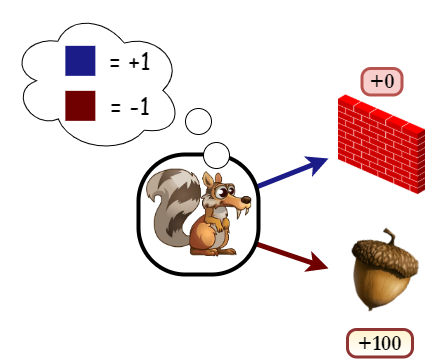
\includegraphics[width=0.28\textwidth]{Images/GreedyIsStupid.png}
\vspace{-0.5cm}
\end{wrapfigure}
\beginproof
Приведём простой пример. Есть два действия: получить приз (+100) и тупить в стену (+0), после выполнения любого игра заканчивается. Заинициализировали $Q^*_0(\text{приз}) \HM= -1$, $Q^*_0(\text{стена}) \HM= +1$. В первой игре, пользуясь текущей аппроксимацией $\pi^*$, выбираем тупить в стену. Получая 0, сглаживаем 0 и текущее приближение +1, получая новое значение $Q^*_{k=1}(\text{стена}) \HM\ge 0$. Оно превосходит $Q^*_{k=1}(\text{приз}) \HM= -1$. Очевидно, и в дальнейших играх агент никогда не выберет приз, и оптимальная стратегия не будет найдена. \qed
\end{theorem}

Действительно, детерминированные стратегии не позволяют получить свойство infinite visitation: многие пары $s, a$ просто приниципиально не встречаются в порождаемых ими траекториях. В частности, из-за неё нельзя ограничиваться рассмотрением только класса детерминированных стратегий, хоть и была доказана теорема \ref{pr:deterministicoptimal} о существовании в нём оптимальной стратегии: мы показали, что для сбора данных --- взаимодействия со средой --- детерминированные стратегии не подходят. Какие подходят?

\begin{theorem}
Любая стратегия, для которой $\forall s, a \colon \pi(a \mid s) > 0$, удовлетворяет условию infinite visitation, то есть с отличной от нуля вероятностью в траектории, порождённой $\pi$, встретится любая пара $s, a$.
\begin{proof}
Для любого $s$ существует набор действий $a_0, a_1 \dots a_N$, которые позволяют с некоторой ненулевой вероятностью добраться до него из $s_0$: $p(s \mid s_0, a_0 \dots a_N) > 0$; если это не так, то ни одна стратегия никогда не попадёт $s$, и мы без ограничения общности можем считать, что таких <<параллельных вселенных>> в нашей среде не существует. Значит, $\pi$ с некоторой ненулевой вероятностью выберет эту цепочку действий $a_0 \dots a_N$, после чего с ненулевой вероятностью окажется в $s$ и с ненулевой вероятностью выберет заданное $a$.
\end{proof}
\end{theorem}

Если мы воспользуемся любой такой стохастической стратегией, мы попадём под действие теоремы о сходимости \ref{th:TDconvergencetheorem}. Совершая случайные действия, мы рискуем творить ерунду, но занимаемся \emph{исследованием} (exploration) --- поиском новых возможностей в среде. Означает ли это, что нам достаточно взять полностью случайную стратегию, которая равновероятно выбирает из множества действий, отправить её в среду порождать переходики $s, a, r, s', a'$, обучать на них Q-функцию и на выходе в пределе мы получим $Q^*$? В пределе --- да.

\begin{example}
Представьте, что вы отправили случайную стратегию играть в Марио. Через экспоненциально много попыток она случайно пройдёт первый уровень и попадёт на второй; для состояний из второго уровня будет проведено первое обновление Q-функции. Через условно бесконечное число таких удач Q-функция для состояний из второго уровня действительно будет выучена...
\end{example}

Иначе говоря, исследование --- корректный, но не эффективный способ генерации данных. Использование --- куда более эффективный метод, позволяющий быстро добираться до <<труднодоступных областей>> в среде --- такими областями обычно являются области с высокой наградой, иначе задача RL скорее всего не является особо интересной --- и быстрее набирать сэмплы для обновлений пока ещё редко обновлённых ячеек $Q^\pi(s, a)$. Но это <<некорректный>> способ: детерминированная стратегия может застрять в локальном оптимуме и никогда не увидеть, что в каком-то месте другое действие даёт ещё большую награду.

Обсудим базовые варианты, как можно решать этот exploration-exploitation trade-off в контексте вычисления оптимальной Q-функции методом временных разностей. Нам нужно взять нашу стратегию использования $\pi(s) \HM\coloneqq \argmax\limits_{a} Q^*(s, a)$ и что-нибудь с ней поделать так, чтобы она стала формально стохастичной.

\begin{definition}
\emph{$\eps$-жадной} ($\eps$-greedy) называется стратегия
$$\pi(s) = \begin{cases}
a \sim \Uniform(\A) & \text{с вероятностью $\eps$;} \\
\argmax\limits_a Q^*(s, a) & \text{иначе.}
\end{cases}
$$
\end{definition}

\begin{definition}
\emph{Больцмановской} с температурой $\tau$ называется стратегия
$$\pi(a \mid s) = \softmax \left( \frac{Q^*(s, a)}{\tau} \right)$$
\end{definition}

Для Больцмановской стратегии мы увидим интересную интерпретацию в контексте обсуждения Maximum Entropy RL (раздел \ref{SACsection}).

\subsection{Q-learning}

Итак, соберём классический алгоритм табличного RL под названием Q-learning. Это метод временных разностей для вычисления оптимальной Q-функции с $\eps$-жадной стратегией исследования.

\begin{algorithm}{Q-learning}
\textbf{Гиперпараметры:} $\alpha$ --- параметр экспоненциального сглаживания, $\eps$ --- параметр исследований

\vspace{0.3cm}
Инициализируем $Q^*(s, a)$ произвольно для всех $s \in \St, a \in \A$ \\
Наблюдаем $s_0$ \\ 
\textbf{На $k$-ом шаге:}
\begin{enumerate}
    \item с вероятностью $\eps$ играем $a_k \sim \Uniform(\A)$, иначе $a_k = \argmax\limits_{a_k} Q^*(s_k, a_k)$
    \item наблюдаем $r_k, s_{k+1}$
    \item обновляем $Q^*(s_k, a_k) \leftarrow Q^*(s_k, a_k) + \alpha \left( r_k + \gamma \max\limits_{a_{k+1}} Q^*(s_{k+1}, a_{k+1}) - Q^*(s_k, a_k) \right)$
\end{enumerate}
\end{algorithm}

Q-learning является типичным представителем off-policy алгоритмов: нам нигде не требовались сэмплы взаимодействия со средой конкретной стратегии. Наша стратегия сбора данных могла быть, вообще говоря, произвольной. В том числе возможно обучение с буфера: допустим, некоторый <<эксперт>> $\pi^{\expert}$ провёл много-много сессий взаимодействия со средой и собрал для нас кучу траекторий. Рассмотрим их как набор переходов. Тогда мы можем, вообще не взаимодействуя больше со средой, провести обучение $Q^*$ с буфера: сэмплируем равномерно переход $(s, a, r, s')$ и делаем обновление ячейки $Q^*(s, a)$ по формуле \eqref{Qlearningupdate}. Что мы тогда выучим?

\begin{definition}
Для данного буфера --- набора переходов $(s, a, r, s')$ --- будем называть \emph{эмпирическим MDP} (empirical MDP) MDP с тем же пространством состояний, действий и функций награды, где функция переходов задана следующим образом:
$$\hat{p}(s' \mid s, a) \coloneqq \frac{N(s, a, s')}{N(s, a)},$$
где $N(s, a, s')$ --- число троек $s, a, s'$, входящих в буфер, $N(s, a)$ --- число пар $s, a$, входящих в буфер.
\end{definition}

\begin{proposition}
При выполнении условий на learning rate, Q-learning, запущенный с буфера, выучит $Q^*$ для эмпирического MDP.
\begin{proof}
Именно из эмпирического распределения $\hat{p}(s' \mid s, a)$ приходит $s'$ в формуле обновления (при равномерном сэмплировании переходов из буфера). Следовательно, для такого MDP мы и выучим оптимальную Q-функцию.
\end{proof}
\end{proposition}

Естественно, если буфер достаточно большой, то мы выучим очень близкую $Q^*$ к настоящей. Ещё более интересно, что Q-learning как off-policy алгоритм может обучаться со своего собственного опыта --- со своего же собственного буфера, составленного из порождённых очень разными стратегиями переходов. 

\begin{definition}
\emph{Реплей буфер} (replay buffer, experience replay) --- это память со всеми собранными агентом переходами $(s, a, r, s', \done)$.
\end{definition}

Если взаимодействие со средой продолжается, буфер расширяется, и распределение, из которого приходит $s'$, становится всё больше похожим на настоящее $p(s' \mid s, a)$; на факт сходимости это не влияет.

\begin{algorithm}{Q-learning with experience replay}
\textbf{Гиперпараметры:} $\alpha$ --- параметр экспоненциального сглаживания, $\eps$ --- параметр исследований

\vspace{0.3cm}
Инициализируем $Q^*(s, a)$ произвольно для всех $s \in \St, a \in \A$ \\
Наблюдаем $s_0$ \\ 
\textbf{На $k$-ом шаге:}
\begin{enumerate}
    \item с вероятностью $\eps$ играем $a_k \sim \Uniform(\A)$, иначе $a_k = \argmax\limits_{a_k} Q^*(s_k, a_k)$
    \item наблюдаем $r_k, s_{k+1}$
    \item кладём $s_k, a_k, r_k, s_{k+1}$ в буфер
    \item сэмплируем случайный переход $s, a, r, s'$ из буфера
    \item обновляем $Q^*(s, a) \leftarrow Q^*(s, a) + \alpha \left( r + \gamma \max\limits_{a'} Q^*(s', a') - Q^*(s', a') \right)$
\end{enumerate}
\end{algorithm}

\subsection{SARSA}

Мы придумали off-policy алгоритм: мы умеем оценивать нашу текущую стратегию ($\argmax\limits_a Q(s, a)$, неявно сидящий внутри формулы обновления), используя сэмплы другой стратегии. Иными словами, у нас в алгоритме различаются понятия \emph{целевой политики} (target policy) --- стратегии, которую алгоритм выдаст по итогам обучения, она же оцениваемая политика, то есть та политика, для которой мы хотим посчитать оценочную функцию --- и \emph{политики взаимодействия} (behavior policy) --- стратегии взаимодействия со средой, стратегии с подмешанным эксплорейшном. Это различие было для нас принципиально: оптимальны детерминированные стратегии, а взаимодействовать со средой мы готовы лишь стохастичными стратегиями. У этого <<несовпадения>> есть следующий эффект.

\begin{exampleBox}[label=ex:cliffworld]{Cliff World}
Рассмотрим MDP с рисунка с детерминированной функцией переходов, действиями вверх-вниз-вправо-влево и $\gamma < 1$; за попадание в лаву начисляется огромный штраф, а эпизод прерывается.

\needspace{7\baselineskip}
\begin{wrapfigure}{r}{0.35\textwidth}
%\vspace{-0.3cm}
\centering
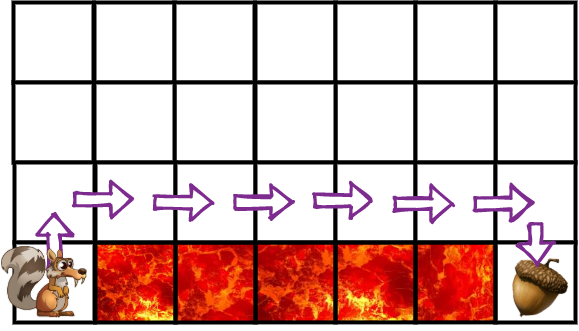
\includegraphics[width=0.3\textwidth]{Images/SafeRL1.png}
%\vspace{-0.3cm}
\end{wrapfigure}
Q-learning, тем не менее, постепенно сойдётся к оптимальной стратегии: кратчайшим маршрутом агент может добраться до терминального состояния с положительной наградой. Однако даже после того, как оптимальная стратегия уже выучилась, Q-learning продолжает прыгать в лаву! Почему? Проходя прямо возле лавы, агент каждый шаг подбрасывает монетку и с вероятностью $\eps$ совершает случайное действие, которое при невезении может отправить его гореть! Если речь не идёт о симуляции, подобное поведение даже во время обучения может быть крайне нежелательно.
\end{exampleBox}

Возможны ситуации, когда небезопасное поведение во время обучение не является проблемой, но для, например, реальных роботов сбивать пешеходов из-за случайных действий --- не самая лучшая идея. Что, если мы попробуем как-то <<учесть>> тот факт, что мы обязаны всегда заниматься исследованиями? То есть внутри оценочной функции должно закладываться, что <<оптимальное>> поведение в будущем невозможно, а возможно только около-оптимальное поведение с подмешиванием исследования. Для примера будем рассматривать $\eps$-жадную стратегию, пока что с константным $\eps$.

Рассмотрим очень похожий на Q-learning алгоритм. Будем использовать пятёрки $s, a, r, s', a'$ (hence the name) прямо из траекторий нашего взаимодействия со средой и апдейтить текущее приближение Q-функции по формуле
\begin{equation}\label{sarsa}
Q(s, a) \leftarrow Q(s, a) + \alpha \left( r(s, a) + \gamma Q(s', a') - Q(s, a) \right)
\end{equation}

Какую Q-функцию такой алгоритм будет учить? Поскольку $a' \sim \pi$, где $\pi$ --- стратегия взаимодействия со средой, то мы стохастически аппроксимируем $Q^{\pi}$, решая явно обычное уравнение Беллмана. Формула обновления не будет эквивалентна формуле Q-learning-а \eqref{Qlearningupdate}: $a'$ мог быть тем самым <<случайным>> действием, случившимся из-за исследований. В большинстве случаев (с вероятностью $1 \HM- \eps$) обновление будет совпадать с Q-learning: тогда $a'$ будет аргмаксимумом, но иногда наша Q-функция будет сдвигаться в сторону ценности случайных действий. Так в оценочную функцию попадает знание о том, что в будущем мы на каждом шаге с вероятностью $\eps$ будем обязаны выбрать случайное действие, и подобное <<дёрганье>> может мешать нам проходить по краю вдоль обрыва с лавой.

\begin{algorithm}{SARSA}
\textbf{Гиперпараметры:} $\alpha$ --- параметр экспоненциального сглаживания, $\eps$ --- параметр исследований

\vspace{0.3cm}
Инициализируем $Q(s, a)$ произвольно для всех $s \in \St, a \in \A$ \\
Наблюдаем $s_0$ \\ 
$a_0 \sim \Uniform(\A)$. \\
\textbf{На $k$-ом шаге:}
\begin{enumerate}
    \item наблюдаем $r_k, s_{k+1}$
    \item с вероятностью $\eps$ играем $a_{k+1} \sim \Uniform(\A)$, иначе $a_{k+1} = \argmax\limits_{a_{k+1}} Q(s_{k+1}, a_{k+1})$
    \item обновляем $Q(s_k, a_k) \leftarrow Q(s_k, a_k) + \alpha \left( r_k + \gamma Q(s_{k+1}, a_{k+1}) - Q(s_k, a_k) \right)$
\end{enumerate}
\end{algorithm}

Попробуем понять формальнее, что происходит в таком алгоритме. Он чередует два шага: обновление \eqref{sarsa}, которое учит $Q^{\pi}$ для текущей $\pi$, и, неявно, некий аналог policy improvement-а: замены $\pi$ на $\eps\operatorname{-greedy}(Q^{\pi})$. Именно при помощи обновлённой стратегии мы будем взаимодействовать со средой на следующем шаге. Является ли такое обновление policy improvement-ом (допустим, для идеально посчитанной $Q^\pi$)? Вообще говоря, нет, но наши стратегии $\pi$, которые мы рассматриваем --- не произвольные. Они все $\eps$-жадные. Введём на минутку такое определение.

\begin{definition}
Будем говорить, что стратегия $\pi$ --- \emph{$\eps$-мягкая} ($\eps$-soft), если $\forall s, a \colon \pi(a \mid s) \HM\ge \frac{\eps}{|\A|}$.
\end{definition}

\begin{proposition}
Если $\pi_1$ --- $\eps$-мягкая, то $\pi_2 \HM\coloneqq \eps\operatorname{-greedy}(Q^{\pi_1})$ не хуже, чем $\pi_1$.
\begin{proof}
Проверим выполнение теоремы \ref{th:policyimprovement}; выглядит немного страшновато, но суть этих выкладок довольно лобовая:
\begin{align*}
V^{\pi_1}(s) &= \{ \text{уравнение VQ \eqref{VQ} } \} = \sum_a \pi_1(a \mid s) Q^{\pi_1}(s, a) = \\
&= \sum_a \left(\pi_1(a \mid s) - \frac{\eps}{|\A|} \right) Q^{\pi_1}(s, a) + \frac{\eps}{|\A|} \sum_a Q^{\pi_1}(s, a) = \\
&= (1 - \eps) \sum_a \frac{\pi_1(a \mid s) - \frac{\eps}{|\A|}}{1 - \eps} Q^{\pi_1}(s, a) + \frac{\eps}{|\A|} \sum_a Q^{\pi_1}(s, a) \le \\
&\le (1 - \eps) \max_a Q^{\pi_1}(s, a) \sum_a \frac{\pi_1(a \mid s) - \frac{\eps}{|\A|}}{1 - \eps} + \frac{\eps}{|\A|} \sum_a Q^{\pi_1}(s, a) = (*)
\end{align*}
Заметим, что последний переход был возможен только потому, что $\pi_1(a \mid s) - \frac{\eps}{|\A|} \HM> 0$ по условию, так как $\pi_1$ --- $\eps$-мягкая по условию. Осталось заметить, что 
$$\sum_a \frac{\pi_1(a \mid s) - \frac{\eps}{|\A|}}{1 - \eps} = \frac{\sum_a \pi_1(a \mid s) - \frac{\eps}{|\A|}}{1 - \eps} = 1,$$
и мы показали, что $V^{\pi_1}(s) \le \E_{\pi_2(a \mid s)}Q^{\pi_1}(s, a)$.
\end{proof}
\end{proposition}

Давайте изменим постановку задачи: скажем, что мы запрещаем к рассмотрению стратегии, <<похожие на детерминированные>>. Наложим ограничение в нашу задачу оптимизации: скажем, что стратегия обязательно должна быть $\eps$-мягкой. В такой задаче будут свои оптимальные оценочные функции.

\begin{definition}
Для данного MDP оптимальными $\eps$-мягкими оценочными функциями назовём:
$$V^*_{\eps\operatorname{-soft}}(s) \coloneqq \max_{\pi \in \eps\operatorname{-soft}} V^{\pi}(s)$$
$$Q^*_{\eps\operatorname{-soft}}(s, a) \coloneqq \max_{\pi \in \eps\operatorname{-soft}} Q^{\pi}(s, a)$$
\end{definition}

\needspace{5\baselineskip}
\begin{wrapfigure}{r}{0.35\textwidth}
\vspace{-0.4cm}
\centering
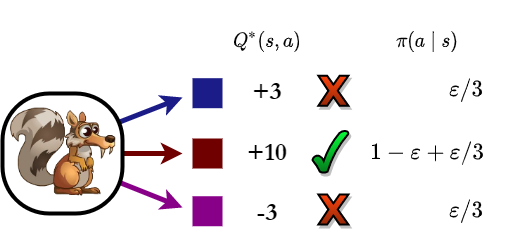
\includegraphics[width=0.35\textwidth]{Images/eSoftBellman.png}
\vspace{-0.8cm}
\end{wrapfigure}

Как тогда будет выглядеть принцип оптимальности? Раньше нужно было выбирать самое хорошее действие, но теперь так делать нельзя. Проводя аналогичные рассуждения, можно показать, что теперь оптимально выбирать самое хорошее действие с вероятностью $1 \HM- \eps \HM+ \frac{\eps}{|\A|}$, а всем остальным действиям выдавать минимально разрешённую вероятность $\frac{\eps}{|\A|}$. Как это понять? Мы уже поняли, что <<взятие $\eps$-жадной>> стратегии есть местный Policy Improvement. Если мы не можем его провести ни в одном состоянии, а то есть $\pi \equiv \eps\operatorname{-greedy}(Q^{\pi})$, то, видимо, придумать стратегию лучше в принципе невозможно:

\begin{proposition}
Стратегия $\pi$ оптимальна в классе $\eps$-мягких стратегий тогда и только тогда, когда $\forall s, a$ таких, что $a \not\in \Argmax Q^{\pi}(s, a)$ верно $\pi(a \mid s) \HM= \frac{\eps}{|\A|}$.
\begin{proof}[Скетч доказательства]
Притворимся, что в будущем мы сможем выбирать действия как угодно $\eps$-мягко, то есть для данного состояния $s$ для каждого действия $a$ сможем в будущем набирать $Q^*_{\eps\operatorname{-soft}}(s, a)$. Как нужно выбрать действия сейчас? Нужно решить такую задачу оптимизации:
$$
\begin{cases}
\E_{\pi(a \mid s)} Q^*_{\eps\operatorname{-soft}}(s, a) \to \max\limits_{\pi} \\
\int\limits_\A \pi(a \mid s) \diff a = 1; \qquad \forall a \in \A \colon \pi(a \mid s) \ge \frac{\eps}{|\A|}
\end{cases}
$$
Формально решая эту задачу условной оптимизации, получаем доказываемое.
\end{proof}
\end{proposition}

\begin{proposition}
Уравнения оптимальности, соответственно, теперь выглядят так:
$$Q^*_{\eps\operatorname{-soft}}(s, a) = r + \gamma \E_{s'} \left[ (1 - \eps) \max_{a'} Q^*_{\eps\operatorname{-soft}}(s', a') + \frac{\eps}{|\A|} \sum_{a'} Q^*_{\eps\operatorname{-soft}}(s', a') \right]$$
\begin{proof}
Их можно получить, например, взяв обычное уравнение QQ \eqref{QQ} и подставив вид оптимальной стратегии.
\end{proof}
\end{proposition}

Мы теперь понимаем, что наша формула обновления \eqref{sarsa} --- просто метод решения такого уравнения оптимальности: сэмплируя $a'$ из $\eps$-жадной стратегии, мы просто стохастически аппроксимируем по мат.ожиданию из $\eps$-жадной стратегии. Мы могли бы, вообще говорять, взять это мат.ожидание полностью явно, сбив таким образом дисперсию:
\begin{align*}\label{expectedsarsa}
Q(s, a) &\leftarrow Q(s, a) + \alpha \left( r(s, a) + \gamma \E_{a' \sim \pi} Q(s', a') - Q(s, a) \right),
\end{align*}
где мат.ожидание по $a'$ по определению $\pi$ равно
$$\E_{a' \sim \pi} Q(s', a') = (1 - \eps) \max_{a'} Q(s', a') + \frac{\eps}{|\A|} \sum_{a'} Q(s', a')$$

Такая схема называется Expected SARSA --- <<SARSA, в которой взяли мат.ожидание>>. Мы всё ещё учим Q-функцию текущей политики, но не используем сэмпл из текущей траектории, а вместо этого берём мат.ожидание по действиям из уравнения Беллмана \eqref{QQ} честно. Вообще говоря, в такой схеме мы работаем не с пятёрками $s, a, r, s', a'$, а с четвёрками $s, a, r, s'$ (несмотря на название).

\begin{algorithm}{Expected-SARSA}
\textbf{Гиперпараметры:} $\alpha$ --- параметр экспоненциального сглаживания, $\eps$ --- параметр исследований

\vspace{0.3cm}
Инициализируем $Q(s, a)$ произвольно для всех $s \in \St, a \in \A$ \\
Инициализируем $\pi_0$ произвольно \\
Наблюдаем $s_0$ \\
\textbf{На $k$-ом шаге:}
\begin{enumerate}
    \item играем $a_k \sim \pi_k(a_k \mid s_k)$
    \item наблюдаем $r_k, s_{k+1}$
    \item $\pi_{k+1}$ есть с вероятностью $\eps$ выбрать $a_{k+1} \sim \Uniform(\A)$, иначе $a_{k+1} = \argmax\limits_{a_{k+1}} Q(s_{k+1}, a_{k+1})$
    \item обновляем $Q(s_k, a_k) \leftarrow Q(s_k, a_k) + \alpha \left( r_k + \gamma \E_{a_{k+1} \sim \pi_{k+1}}Q(s_{k+1}, a_{k+1}) - Q(s_k, a_k) \right)$
\end{enumerate}
\end{algorithm}

Соответственно, и SARSA, и Expected SARSA будут сходиться уже не к обычной оптимальной оценочной функции, а к $Q^*_{\eps\operatorname{-soft}}(s, a)$ --- оптимальной оценочной функции в семействе $\eps$-мягких стратегий.

\begin{exampleBox}[righthand ratio=0.35, sidebyside, sidebyside align=center, lower separated=false]{Cliff World}
Попробуем запустить в MDP из примера \ref{ex:cliffworld} SARSA. Мы сойдёмся вовсе не к оптимальной стратегии --- а <<к безопасной>> оптимальной стратегии. Внутри нашей оценочной функции сидит вероятность сорваться в лаву при движении вдоль неё, и поэтому кратчайший маршрут перестанет давать нам наибольшую награду просто потому, что стратегии, для которых такой маршрут был оптимален, мы перестали допускать к рассмотрению.

\tcblower
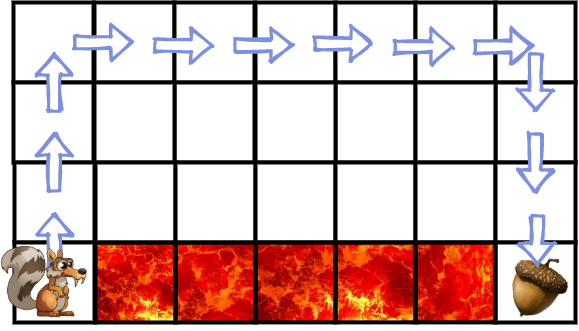
\includegraphics[width=\textwidth]{Images/SafeRL2.png}
\end{exampleBox}

Принципиальное отличие схемы SARSA от Q-learning в том, что мы теперь учимся ровно на тех же сэмплах действий $a'$, которые отправляем в среду. Наши behavior и target policy теперь совпадают: для очередного шага алгоритма нужно сделать шаг в среде при помощи текущей $\pi$, и поэтому мы должны учиться онлайн, <<в on-policy режиме>>.

Чтобы понять, что это влечёт, рассмотрим, что случится, если взять буфер некоторого эксперта $\pi_{\expert}$, генерировать пятёрки $s, a, r, s', a'$ из него и проводить обновления \eqref{sarsa} по ним. Что мы выучим? Применяем наш стандартный ход рассуждений: $a' \HM\sim \pi_{\expert}(a' \mid s')$, и, значит, мы учим $Q^{\expert}$! Если же мы попробуем запустить SARSA с experience replay, то есть обучаться на собственной же истории, то мы вообще творим полную фигню: на каждом шаге мы движемся в сторону Q-функции для той стратегии $\pi$, которая породила засэмплированный переход (например, если переход был засэмплирован откуда-то из начала обучения --- скорее всего случайной или хуже). Такой алгоритм не просто будет расходиться, но и не будет иметь никакого смысла. Поэтому SARSA нельзя (в таком виде, по крайней мере) запустить с реплей буфера.

% Похоже, можно по-разному договариваться, что значит использовать буфер в этой схеме. Из буфера берутся четвёрки $s, a, r, s'$, а дальше возникает разное понимание, по $a'$ из какого распределения брать мат.ожидание в формуле. рассмотрим все варианты. Например, технически, если мат.ожидание $\E_{a'}$ берётся по вероятностям, использовавшимся для выбора действия экспертом, собиравшим опыт (и заодно записывавшим свои вероятности выбора действий, чтобы мы могли такое мат.ожидание брать), то мы учим потенциально неоптимальный $Q^{\pi_{\expert}}$. Такая схема, понятно, on-policy. Если мы берём мат.ожидание $\E_{a'}$ всегда по текущей версии стратегии и используем жадную стратегию $a' = \argmax\limits_{a'} Q(s', a')$, то формально мат.ожидание вырождается, и мы получаем Q-learning (он в чистом виде off-policy). 

% Кажется, наиболее каноничный вариант --- брать мат.ожидание по текущей версии стратегии $\pi_{k+1}$, с учётом эксплорейшна: тогда мы для любой четвёрки $s, a, r, s'$ движемся к $Q^{\pi_{k+1}}$, алгоритм представляет собой Policy Iteration в классе $\eps$-аугментированных стратегий, который для любого буфера сходится, условно говоря, к оптимальной $\eps$-аугментированной стратегии. В последнем варианте, на мой взгляд, возможность использования произвольного буфера даёт основание относить алгоритм к off-policy, но в некоторых источниках почему-то пишут on-policy из-за сходимости не к оптимальной $Q^*$.

% Итого, является ли Expected-SARSA on-policy или off-policy, мы к консенсусу не пришли.